
\documentclass[phd,tocprelim]{cornell}

\let\ifpdf\relax
\usepackage{url}
\usepackage{graphicx}
\usepackage{float}
\usepackage{color}

\usepackage[section]{placeins}
\usepackage{graphicx,pstricks}
\usepackage{graphics}

\usepackage{moreverb}
\usepackage{subfigure}
\usepackage{epsfig}
\usepackage{subfigure}
\usepackage{txfonts}
\usepackage{subcaption}
\usepackage{multirow}
\usepackage{todonotes}
\usepackage{glossaries}


\graphicspath{ {Images/} }

\usepackage[utf8]{inputenc}


\tolerance=9999

\bibliographystyle{plain}
%\bibliographystyle{IEEEbib}

\usepackage{listings}
\usepackage{color}

\makeglossaries


\definecolor{dkgreen}{rgb}{0,0.6,0}
\definecolor{gray}{rgb}{0.5,0.5,0.5}
\definecolor{mauve}{rgb}{0.58,0,0.82}
\renewcommand{\topfraction}{0.85}
\renewcommand{\textfraction}{0.1}
\renewcommand{\floatpagefraction}{0.75}
\usepackage{hyperref}

\title{Forbedret brukervennlighet innen alternativ og supplerende kommunikasjon for mennesker med forsinket 
eller avvikende språk- og kommunikasjonsutvikling.} 
\author{Morten Holst Øvrebø}

\begin{document}

\begin{figure}[ht!]
\centering

\includegraphics[width=80mm]{HIB_sort_hovedlogo_engelsk}
\end{figure}


\maketitle
\begin{abstract}
Abstract here.
\end{abstract}

\begin{acknowledgements}
acknowledgements here. 
\end{acknowledgements}

\newglossaryentry{isaac}{name=ISAAC, description={ International Society for Augmentative and Alternative Communication}}

 \newglossaryentry{aske}{name=ASK, description={alternativ og supplerende kommunikasjon}}
 
 
  \newglossaryentry{PCCR}{name=PCCR, description={Pupil Centre Cornea Reflection, er en teknikk som brukes til ikke-forstyrrende øyesporing}}


  \newglossaryentry{WPF}{name=WPF, description={Windows  Presentation  Foundation}}


 
\printglossaries
\contentspage
\figurelistpage
\listoftodos

\normalspacing \setcounter{page}{1} \pagenumbering{arabic}
\pagestyle{cornell} \addtolength{\parskip}{0.5\baselineskip}



\chapter{Introduksjon}




\section{Motivasjon}
\label{sec:motivasjon}

Tale og språk tillater oss å rekke ut til andre og leve tilfredstillende liv som uavhengige medlemmer av samfunnet. Språk gir oss identitet, felleskap  og tilhørighet. Det er derimot flere som blir hindret i å uttrykke seg gjennom tradisjonelle kommunikasjonsformer, enten ved funksjonshemning eller skade  \cite{tobii}. Gjennom århundrer har denne samfunnsgruppen hatt behov for alternativer for å kunne kommunisere. Folk med syn eller hørselsskader har tatt i bruk gester, tegnstøtte eller tegnspåk. Andre har måttet bruke mer håndgripelige hjelpemidler. Ett kjennetegn ved disse formene for kommunikasjon er at de krever at brukeren har muskelkraft. Personer med ALS, Cerebral Parese, utviklinghemming, autisme og Afasi eller hjerneslag har ofte motoriske utfordringer som hindrer dem fra nettopp verbal og kroppspråklig kommunikasjon. Ved hjelp av data- og øyestyrings-teknologi er det mulig for flere av disse menneskene å kommunisere. Utfordringen er at feltet er relativt ungt og nåværende forskning har en tendens til å reflektere konseptuelle modeller og prioriterer voksne uten funksjonshemninger \cite{aac}. I dette prosjektet vil fokus bli rettet mot barn som ikke har tilgang på tradisjonelle kommunikasjonsformer.




\section{Målgruppe}

I kapittel \ref{sec:motivasjon} nevnes det at det er flere unge mennesker som helt eller delvis mangler tale. Som en konsekvens av dette har de behov for andre uttrykksformer for å kommunisere. Alternative uttrykksformer kan være håndtegn, symboler eller fotografier. Slike utradisjonelle uttrykksformer går under fellesbetegnelsen alternativ og supplerende kommunikasjon (\gls{aske}).
Personer bruker ASK enten fordi det er et behov for å erstatte talen eller for å supplere talen på grunn av at den er for utydelig eller svak. 

Der alternativ kommunikasjon er for mennesker som har behov for å erstatte talen. Supplerende for mennesker som har tale, men som er utydelig eller for svak og har derfor behov for støtte til å kommunisere.  International Society for Augmentative and Alternative Communication (\gls{isaac}) \cite{HvaErASK} definerer ASK som alt som hjelper en person til å kommunisere effektivt når tradisjonelle måter å kommunisere på ikke strekker til.  

I denne avhandlingen vil den  målgruppen være mennesker som har behov for  ASK systemer. Området er derimot veldig stort og brukerene har svært forskjellige behov og utgangspunkt. Mer spesifikk vil den rapporten være rettet mot: (A) Mennesker som ikke har mulighet for tale- og kroppspråk,  (B) personer ikke håndterer skriftspråk og (C) barn i alderen 2 til 5 år og eldre med mentale begrensninger. Fellesnevneren er at de er nybegynnere på symbolbasert kommunikasjon. Videre i dette prosjektet vil personer som møter disse kriteriene bli omtalt som barn med komplekse kommunikasjonsbehov. 

\section{Mål}
\label{sec:goal}

Målet med dette prosjektet er å lage et ASK system som hjelper barn med komplekse kommunikasjonsbehov å kommunisere. Systemet som skal utvikles skal tar utgangspunkt i et eksisterende program som heter Sono Flex(se figur ~\ref{fig:SonoFlex}). Programmets hovedfunksjon er å konvertere tekst og symboler til tale, samt at det innholder et rikholdig utvalg av funksjoner for læring, omgivelsekontroll og elektronisk fjernkommunikasjon \cite{TobiiCommunicator}. Hovedfunksjonen er at systemet hjelper brukeren å kommunisere ved bruk av symboler. Der et symbol representerer et ord eller et konsept som "hjem" eller "min mor". Problemstillingen er at når brukerens aktive vokabular vokser, så vil også antallet symboler øke. Dette gjør at det oppstår et behov for å dele symbolene inn i kategorier og flere visninger.

Light og Drager \cite{aac} argumenterer at videre forskning innen ASK teknologi må fokusere på forbedret design, for å bedre kunne møte behovet fra unge barn og eldre nybegynnere. I dette prosjektet er målet å designe og prototype mulige løsninger som reduserer den mentale belastningen på brukeren. Mens hun opererer a stort vokabular med eller uten en øyestyrings enhet.

\begin{figure}[ht!]
\centering
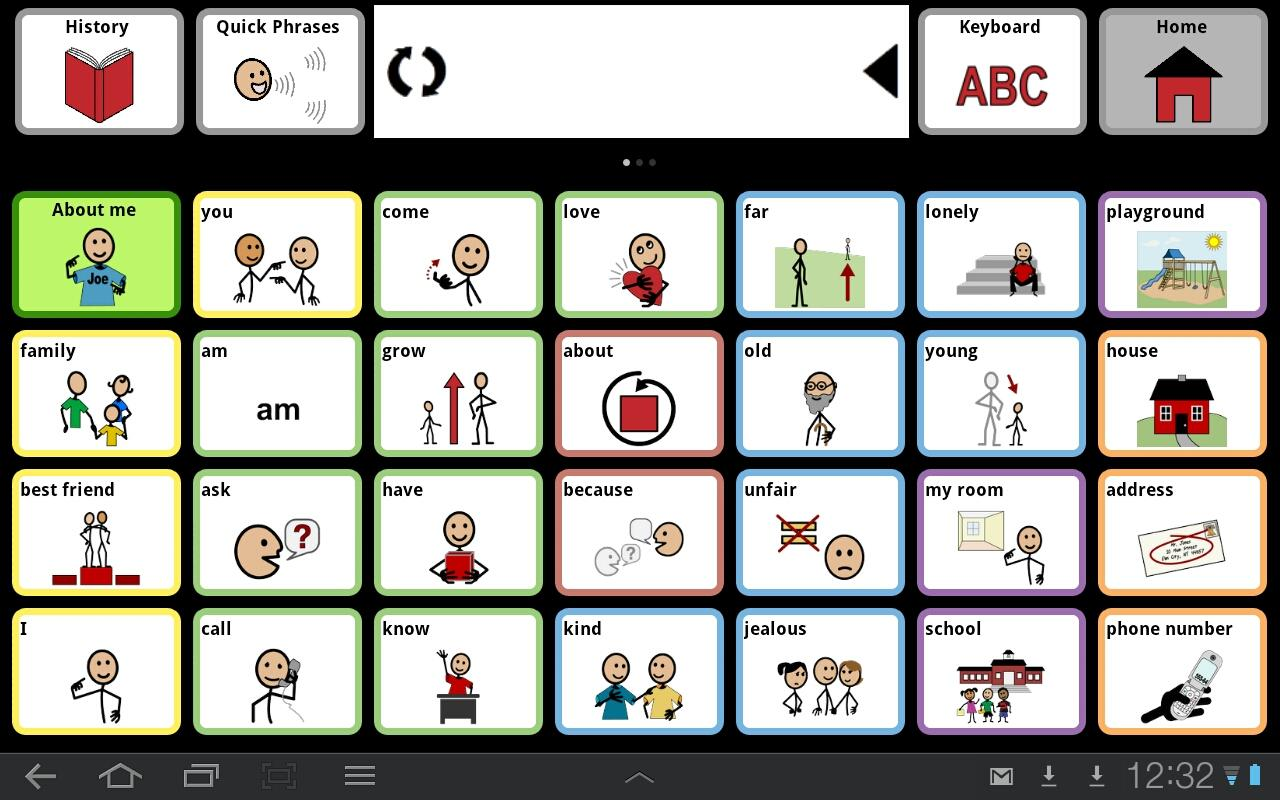
\includegraphics[width=150mm]{SonoFlex2}
\caption{Skjermdump av ASK programvaren Sono Flex}
\label{fig:SonoFlex}
\end{figure}


\section{Forskningspørsmål}
\label{sec:ResearchQuestion}

For å forske på mulige løsninger som forbedrer ASK systemer vil en rekke funksjoner integreres i prototypen. Funksjoner som vil bli utprøvd og forsket på er listet i \ref{lst:features}.


\begin{enumerate} 
\label{lst:features}
\item Forbedret visualisering. Undersøk mulige fordeler forskjellige visualisering effekter kan ha på navigering innen og mellom sider og kategorier.
\item Lyd effekter. Undersøk mulige fordeler forskjellige lyd effekter kan ha på navigering innen og mellom sider og kategorier.
\item Optimal organisering og kategorisering. Hvordan skal knapper bli organisert og kategorisert for å best legge til rette for og simplifisere navigasjon
\item Brukertilpasning. Mennesker har forskjellige preferanser. Gjelder dette også for symbolstørrelse, animasjonsfart, hurtighet o.s.v. Undersøk fordelene.  
\end{enumerate} 


Forskningen vil bli gjort ved å implementere et program basert på en eksisterende løsning. De ulike forbedringene beskrevet i (1),(2) og (3) vil bli integrert. Samtidig vil det også være mulighet tilpasse etter ønske (4). 


\section{Forskningsmetode}

Som nevnt i seksjon \ref{sec:ResearchQuestion}, er oppgaven å forbedre en type kommunikasjons programvare for mennesker med komplekse kommunikasjonsvansker. For å undersøke innvirkningene til de forskjellige funksjonene, vil de prøves ut på en testgruppe.
For å få til dette, vil et utvalg av deltakerene prøve systemet uten tilleggsfunksjonene, mens de gjenværende vil forsøke med funksjonene. Mens deltagerne kjører programmet vil de overvåkes av datamaskinen. informasjonen fra undersøkelsen vil vise hvordan brukeren navigerte og hvor lang tid de brukte. Dette kan igjen brukes til å verifisere om en funksjon er en forbedring eller ikke.


\chapter{Bakgrunn}

Dette kapittelet skal gi leseren en godt fundament for resten av avhandlingen, ved å beskrive de viktigste konseptene, fenomenene og teknologiene. Kapittelet går også inn på tidligere relevant forskning på fagfeltet. 

\section{Kommunikasjonsform: Symboler}

De som ikke har mulighet til å bruke tale som kommunikasjonsform kan bruke tegnsystemer. Det eksisterer tre typer tegnsystemer: håndtegn(manuelle tegn) som innebærer å bruke håndbevegelser, materielle tegn vil si at en bruker fysiske objekter som brikker eller figurer og den siste er; grafiske tegn som innebærer at en bruker symboler. I denne rapporten er det kun vil grafiske tegn bli brukt som kommunikasjonsform. Der symboler representerer et ord, frase, uttrykk eller setning. Ifølge ISAAC \cite{Tegnsystemer} er grafiske tegn brukt av mennesker med store bevegelsesvansker som gjør at de har utfordringer med å lage manuelle tegn, og mennesker med forståelsesvansker som følge av lærehemning.

De vanligste grafiske tegnsystemene på markedet er fotografi, pictogram, picture communication symbols(PCS), Widgit, SymbolStix og Bliss \cite{GrafiskTegn}. I prosjektet brukes tegnsystemet SymbolStix (se figur \ref{fig:katt}). Grunnen til dette er at Sono Flex bruker dette tegnsystemet. For å kunne sammenligne de to er det naturlig å bruke de samme symbolene.


\begin{figure}[ht!]
\centering
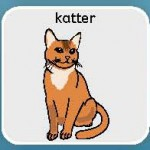
\includegraphics[width=50mm]{katt}
\caption{Et eksempel på et symbol som blir brukt i det grafisk tegnsystemet SymbolStix}
\label{fig:katt}
\end{figure}

\section{Interaksjonsform: Øyestyring}

Menneske-maskin-interaksjon fungerer ved at en person gir maskinen en kommando, og maskinen svarer med en respons. For at et menneske skal kunne gi en maskin ordre, er det nødvendig at maskinen har en inputenhet som tolker  Som regel er dette tradisjonelle enheter som tastatur og mus. Det eksisterer derimot mangfoldige måter å samhandle med en maskin på. Blant så kan en bruke en mikrofon som oversetter stemme til maskinspråk. I denne rapporten vil brukerinput bli gitt ved en øyestyringsenhet.  Ved å fange opp brukerens skuepunkt av et videokamera og infrarøde lys, er det mulig for maskinen å beregne hvor på monitoren personen ser. Dette gjør interaksjon mellom dem mulig. En knapp vil for eksempel bli aktivisert ved at brukeren ser på den et gitt tidspunkt. 




\section{Forskning}


\subsection{Organisering}


I 1926 kartla Smith\cite{Smith} barns vokabularutvikling fra alderen 1 til 5 år . Resultatene (se tabell \ref{fig:BarnVak}) fra undersøkelsen viste at allerede i en alder av 3 er det vanlig å ha forståelse for 896 ord. Forskningen er 88 år gammel, men viser omfanget av utfordringen barn har i møte med symbolbasert kommunikasjon. Mens et barn med taleevne kun trenger å finne ordet i hukommelse, må barn som bruker symboler først finne ordet i hukommelsen og deretter finne det representative symbolet. 

Antall Symboler som kan vises på en side begrenses av skjermens fysiske størrelse - samt at de må være store nok til at brukeren har mulighet til å se  og samhandle med dem. Slik at for hver beskjed må brukeren navigere seg igjennom en tabell for å finne ønsket symbol. Det er derfor essensielt at organiseringen legger til rette for akkurat dette, og ikke vanskeliggjør barnets evne til å lokalisere, velge og bruke konseptene.

\begin{table}[h]
\begin{tabular}{llllllllll}
\hline
Alder (År, Måneder) & 1 & 1,6 & 1,9 & 2,0 & 2,6 & 3,0 & 3,6  & 4,0  & 5,0  \\ 
Antall ord          & 3 & 22  & 118 & 272 & 446 & 896 & 1222 & 1540 & 2072 \\ 
Økning              & 2 & 19  & 96  & 154 & 174 & 450 & 326  & 330  & 532  \\ \hline
\end{tabular}
\caption{Tabell som viser vokabular vekst hos barn.  Smith \cite{Smith} sitert av Dale \cite{Dale} }
\label{fig:BarnVak}
\end{table}



Drager og Light \cite{aac} viser til at det inntil nylig var gjort lite forskning på effektive layouts og organisering eller om faktorene som spiller inn når det gjelder lokalisering og bruk av målobjektene.  Wilkinson og Jageroo \cite{Wilkinson2006} har undersøkt hvilke påvirkning farge har som en faktor når det kommer til organisering og hvordan elementer skal fordeles. De kom frem til at farge hint spiller en viktig rolle innen visuell prosessering  og hukommelse. Ved å legge til en farge ved elementene i tabellen over symboler, påvirket nøyaktigheten og effektiviteten til barn i 4-5 års alderene i å finne målobjekt. Fenomenet  kommer av at når et målobjektets stimulus er distinkt og annerledes fra annen stimuli, vil barn mer presist og raskere lokalisere målobjektet. Målobjektet er symbolet som brukeren ønsker å uttrykke. Scally \cite{Scally} argumenterer for at farge ikke nødvendigvis er den eneste variabelen som må vurderes. Andre skjerm variabler som kan påvirke læring og bruk er: bakgrunn, kanter/grenser, form, tekstur, størrelse, posisjon, bevegelse og animasjon. Videre undersøkelser må til for å avgrense effektene av disse funksjonene for å kunne optimere designet til ask teknologier.


\subsection{Navigasjon}
\label{subsec:navigasjon}

Ettersom et barns vokabular kan bli stort må nødvendigsvis symbolene som representerer ordene deles opp over flere sider. Konsekvensen er at brukeren må ha mulighet til å navigere mellom disse sidene for å finne ønsket symbol. Siden antallet symboler det er plass til på hver side begrenses av skjermstørrelsen og brukerens syn, er spørsmålet hvor mange symboler bør plasseres på hver side med tanke på effektivitet. Drager og light med kollega-er undersøkte nettopp dette på. Resultatene indikerte at barn i alderen 2-5 hadde større vanskeligheter for å lokalisere korrekt side fra en meny med 4 symboler enn en så lokalisere målobjektet når på korrekt side ut av et valg på 12 til 30 symboler, til tross for at sannsynligheten for å finne korrekt side er 25 prosent er mye større enn å finne korrekt symbol 0.03 - 0.08 når en først er på rett side.

For barn kan det å navigere være ekstra vanskelig. Dette kommer av flere grunner: (a) de må ha en konseptuellmodell av de gjemte sidene i systemet i minnet; og (b) de må forstå forholdet mellom representasjon brukt på menysiden og de gjemte sidene i vokabularet. Er det symbolet som har bilde av et kjøkken eller av en butikk som leder til symbolet eple? I denne rapporten vil disse utfordringene bli undersøkt.




\chapter{Øyesporing}

Øyesporing refereres ofte til teknikken brukt til å fange og måle øyebevegelser \cite{Calibration}. Målet med dette kapittelet er å gi en beskrivelse av hvordan øyesporing fungerer og enheten som brukes i denne avhandlingen - samt en forklaring av viktige konsepter.


\section{Hvordan fungerer øyet?}

Å forklare hvordan øyet fungerer i detalj er utenfor denne rapportens omfang. Det vil derfor kun gis en høynivå forklaring av hvordan det fungerer for å kunne forstå det som er nødvendig i henhold til rapporten. 

\subsection{Synsfelt}

I en artikkel skrevet av Tobii \cite{Calibration} sammenlignes øyet med et fotoapparat på grunn av ens mange likhetstrekk. Lys reflekteres fra et objekt - lyset reiser så gjennom en linse å ender opp i øyet. Linsen prosjekterer lyset den mottar på en lyssensitiv overflate. Denne overflatens oppførsel er også det som skiller øyet fra fotoapparatet. For imotsetning til et kamera er ikke overflaten like sensitiv overalt hos øyet. Noe som gjør at menneske kan tilpasse synet etter hvor mye lys som er tilgjengelig. Nedsiden er at det også resulterer i at menneske kun kan se klart i begrensede områder av synsfeltet. Figur \ref{fig:visueltArea} illustrerer hvordan synsfeltet hos menneske er delt inn etter klarhet. (F) representerer det foveale området. Dette er området man fokuserer på og oppfatter klarest. Det er hovedsaklig fra dette området visuell data hentes fra . (Pf) viser det parafovela omårdet, å kjennetegnes ved at uskarpheten øker til man kommer til det perifere området. (P) Det perifere området, også kjent som sidesynet, fungerer kun bra til å fange opp bevegelser og kontraster.

\begin{figure}[ht!]
\centering
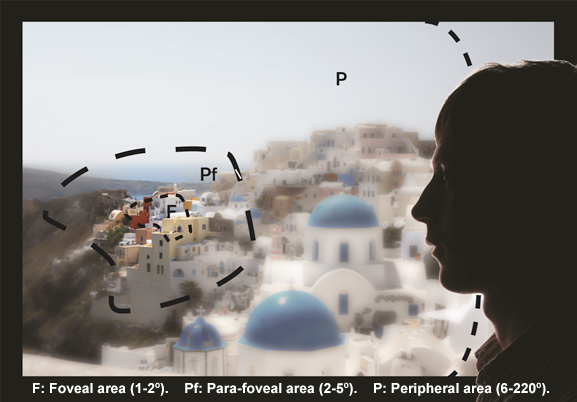
\includegraphics[width=65mm]{fovealArea}
\caption{Bilde/Illustrasjon av menneskelige synsfelt \cite{VisualImage}}
\label{fig:visueltArea}
\end{figure}

\subsection{Fikseringer og sakkader}

Det foveale området er som nevnt det området det registreres mest visuell data. Området står derimot for mindre 8 prosent av synsfeltet. Dette gjør at for å kunne innhente informasjon av interesse fra andre deler av synsfeltet må det flyttes inn i  det foveale området. For å gjøre det brukes øyeoperasjoner kalt fikseringer og sakkader. Fikseringer er pauser fra bevegelsen på et område, sakkader er hurtige bevegelser mellom fikseringene \cite{Calibration}.


\section{Hvordan fungerer øyesporing?}

Øyesporing er som tidligere nevnt teknikken brukt til å fange og måle øyebevegelser.
Det finnes derimot flere fremgangsmåter. I denne oppgaven vil det brukes en ikke-forstyrrende øyestyringsenhet. Som vil si at en bruker i prinsippet ikke vil legge merke til enheten. For denne typen øyesporing er det mest vanlig å bruke en teknikk som heter Pupil Centre Cornea Reflection (\gls{PCCR}) \cite{Calibration}. Teknikken fungerer ved at en lyskilde belyser øyet, dette gir en klare og synlige refleksjoner. Et kamera tar deretter bilde av refleksjonene fra øyet. Bildet blir så brukt til å identifisere lysets refleksjon på hornhinnen og pupillen. Når en vet vinkelen mellom hornhinnen og pupillen er det mulig å regne ut en vektor. Vektoren sammen med andre geometriske egenskaper ved refleksjonene gjør det mulig å kalkulere ut blikkretningen(Der brukeren ser) \cite{Calibration}.


\subsection{Utfordringer}

En utfordring ved øyesporing er blunking. Blunking er et er en kortvarig sammentrekning av øyelokket, noe som gjør at øyet ikke vil gi refleksjon som kamera kan fange, og derfor ikke ha koordinater på hvor brukeren ser. Dette løses under analysen. Ved at man vet koordinatene og fart før øyelokkene trakk seg sammen kan man ekstrapolere seg fram til en tilnærmet korrekt fiksering. 

\section{Tobii PCEye Go}

I denne rapporten brukes øyesporingsenheten Tobii PCEye GO, som vist i figur \ref{fig:tobiiPc}. Enheten kommer separat og kobles til datamaskinen via USB. Dette er som tidligere nevnt et ikke-forstyrrende apparat. Et eksempel på det motsatte ville vært et par briller som ble brukt til å spore øyebevegelser. 



\begin{figure}[ht!]
\centering
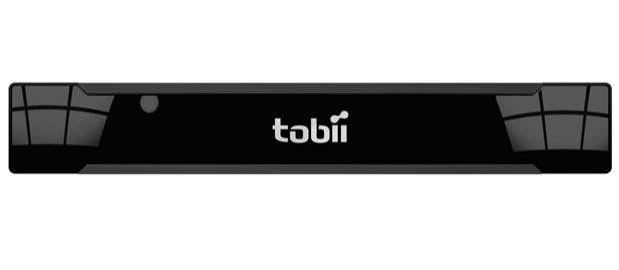
\includegraphics[width=50mm]{TobiiEyeGo}
\caption{Bilde av øyestyringsenheten Tobii PCEye Go}
\label{fig:tobiiPc}
\end{figure}


\subsection{Tobii blikkprogramvare}
\label{subsec:blikk}

Sammen med Tobii PCeye go følger det med programvare for å kontrollere applikasjoner som bruker sporingsenheten. Den består av følgende komponenter: 

\begin{itemize}
\item [Blikk interaksjonsserver] en sentral HUB som tilbyr klient applikasjoner øyesporingsdata. 
\item [Blikk interaksjons innstillinger] Et kontrollpanel for interaksjons innstillinger og oppgaver relatert til øyesporing
\item [Windows Kontroll] Tilbyr blikk interaksjon for standard Windows applikasjoner, ergo vanlige applikasjoner som ikke er laget for øyesporings interaksjon.
\end{itemize}

I denne rapporten vil kun førstnevnte være relevant. Ettersom applikasjonen er spesialisert til blikk interaksjon og ikke er en standard Windows applikasjon.

\subsection{Blikk Interaksjonsserver}

Blikk interaksjons-serveren er som nevnt i seksjon \ref{subsec:blikk} en HUB for programvaren, eller kjernen. Hovedformålet til denne komponenten er å samhandle med Øye-sporingsenheten og tilby interaksjonsfunksjonalitet for å kontrollere Windows baserte applikasjoner som vil bruke sporingsdata. I tilegg er det denne komponenten som tar seg av kalibrering, sporingsstatus - samt bruker og applikasjons innstillinger.

\subsection{Tobii Eye Control API }

Figur \ref{fig:overview} viser hvordan blikk interaksjonsserveren eksponerer funksjonalitet til en klient-applikasjon gjennom et APIet, som er kalt Tec API. For å ta i bruk TecAPIet tilbys to aksess punkter. Et gjennom .NET plattformen kalt TecClient og et for C dynamisk link library kalt MPACI.  Den praktiske betydningen, er at man kun kan bruke APIet ved å skrive i C eller .NET teknologier. I denne rapporten vil kun sistnevnte være interessant, altså .NET APIet kalt TecClient.


\begin{figure}[ht!]
\centering
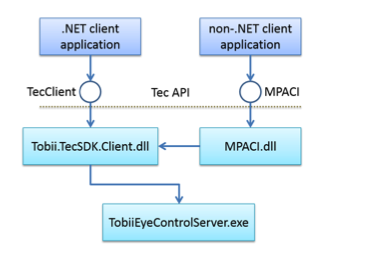
\includegraphics[width=100mm]{SoftwareArchitectureOverview}
\caption{Bilde som viser programvare arkitekturen til blikk programvaren}
\label{fig:overview}
\end{figure}


\subsection{TecClient}

TecClient støtter to GUI rammeverk; Windows Presentation Foundation (\gls{WPF}) og Windows Forms. 
\cite{Dokumentasjonen} (kilde dokumentasjon).  Samhandling mellom applikasjonen og TecClienten skjer gjennom et konsept som de har valgt å kalle TecClients verktøykasse. De ulike verkøys klassene er presentert i figur \ref{fig:toolbox}. 

\begin{figure}[ht!]
\centering
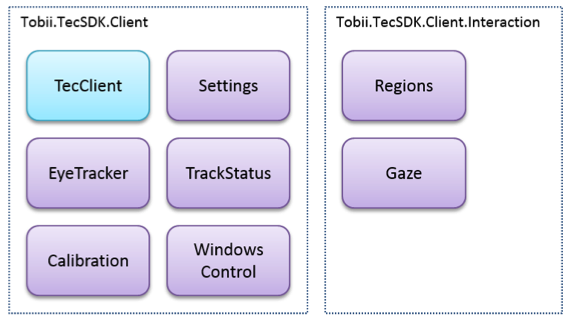
\includegraphics[width=100mm]{Toolbox}
\caption{Verktøy klassser som er tilgjengelige gjennom TecClient komponenten verktøyskasse}
\label{fig:toolbox}
\end{figure}


\subsubsection{EyeTracker}
Gir informasjon om den aktuelle øyesporingsenheten.

\subsubsection{Kalibrering}
Tilbyr tilgang til kalibrerings funksjonalitet og innstillinger som kan bli brukt for å kontroller hvordan kalibreringen er gjort.

\subsubsection{Settings}
Settings gir tilgang til bruker og klient innstillinger. Med mulighet til å hente nåværende bruker, alle bruker med funksjonalitet til å legge til og fjerne brukere og nåværende klient.

\subsubsection{Trackstatus}
Tilbyr metoder, egenskaper og hendelser for å kontrollere sporingsstatus vinduet. 


\subsubsection{Regions}
Tilbyr metoder, egenskaper og hendelser relatert til interaksjonsregioner. (1) Legge til og fjerne interaksjonsregioner, (2) hente informasjon om fokus og (3) søke etter interaksjonsregioner.

\subsubsection{Gaze}
Eksponerer blikkdata, både filtrert og ufiltrert. 


\chapter{Tobii Sono Flex}

I dette kapittelet vil den eksisterende løsningen sono flex bli diskutert. Det vil bli gitt en grundig analyse av problemstillingen og fremgangsmåte presentert.


\section{Tobii Sono Flex}
\label{chap:Tobii-Sono-Flex}


Programvaren som det tas utgangspunkt i heter Tobii Sono Flex,  og er et systematisert symbolforråd og et verktøy for alternativ og supplerende symbolspråk.  Der bilder gjøres om til tydelig tale og tilbyr et språk til personer som ikke enda kan lese og skrive (kilde tobii). Systemet er spesielt utviklet for barn og unge med med sammensatte kommunikasjonsvansker, som trenger et ordforråd for å videreutvikle språk- og kommunikasjonsferdigheter. Sono flex kan ses på som en nybegynnerpakke med en lav læringskurve. Som skal gjøre brukeren klar for mer avanserte systemer. 


\subsection{Brukergrensesnitt}

Brukergrensesnittet til Sono Slex består av to hovedkomponenter: en menylinje og en symbolgrid. 


\subsubsection{Menylinje}

Figur \ref{fig:menylinje} viser menylinjen.  Denne består av 5 elementer; der de to ytterste,  word magic og more contexts er dynamiske og vil endres, og er ikke videre interessant for denne rapporten.  De gjenværende er statiske og følger applikasjonen hele tiden. Det hvite feltet i midten viser symbolene som brukerene har trykket på, og vil herved bli referert til som inndatafeltet. Symbolene som vises vil komme ut i form av tydelig tale ved å trykke på selve feltet. Knappen på venstre side av inndatafeltet (clear all), vil ved interaksjon tømme inndatafeltet. Mens knappen på høyre side vil kun fjerne det siste symbolet brukeren trykket på.


\begin{figure}[ht!]
\centering
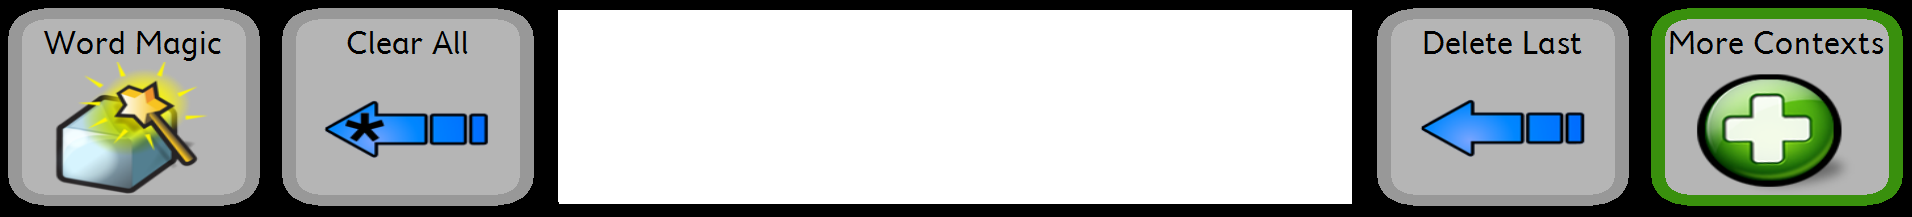
\includegraphics[width=100mm]{menylinje}
\caption{Skjermdump av menylinjen til programvaren Sono Flex}
\label{fig:menylinje}
\end{figure}




\subsubsection{Symbolgrid}

Figur \ref{fig:symbolgrid} viser applikasjonens symbolgrid. Dette komponentet består av en tabell på 7 kolonner og 4 rader,  noe som gir 28 celler. I hver celle er det et Knapp bestående av et symbol og en tekstlig beskrivelse av symbolet. Ved å trykke på knappen vil en av to ting skje avhengig av hvilken type knappen er av. Hvis knappen representerer et ord( "jeg",  "løpe",  "kake" o.s.v. ) så vil symbolet og medfølgende tekst vises i inndatafeltet i menylinje.  Hvis knappen har underliggende knapper som eksempelvis ordklasse(verb,  substantiv)  eller kategori ("mat",  "frukt") så vil applikasjonen bytte ut de eksisterende knappene i tabellen med de underliggende. 


\begin{figure}[ht!]
\centering
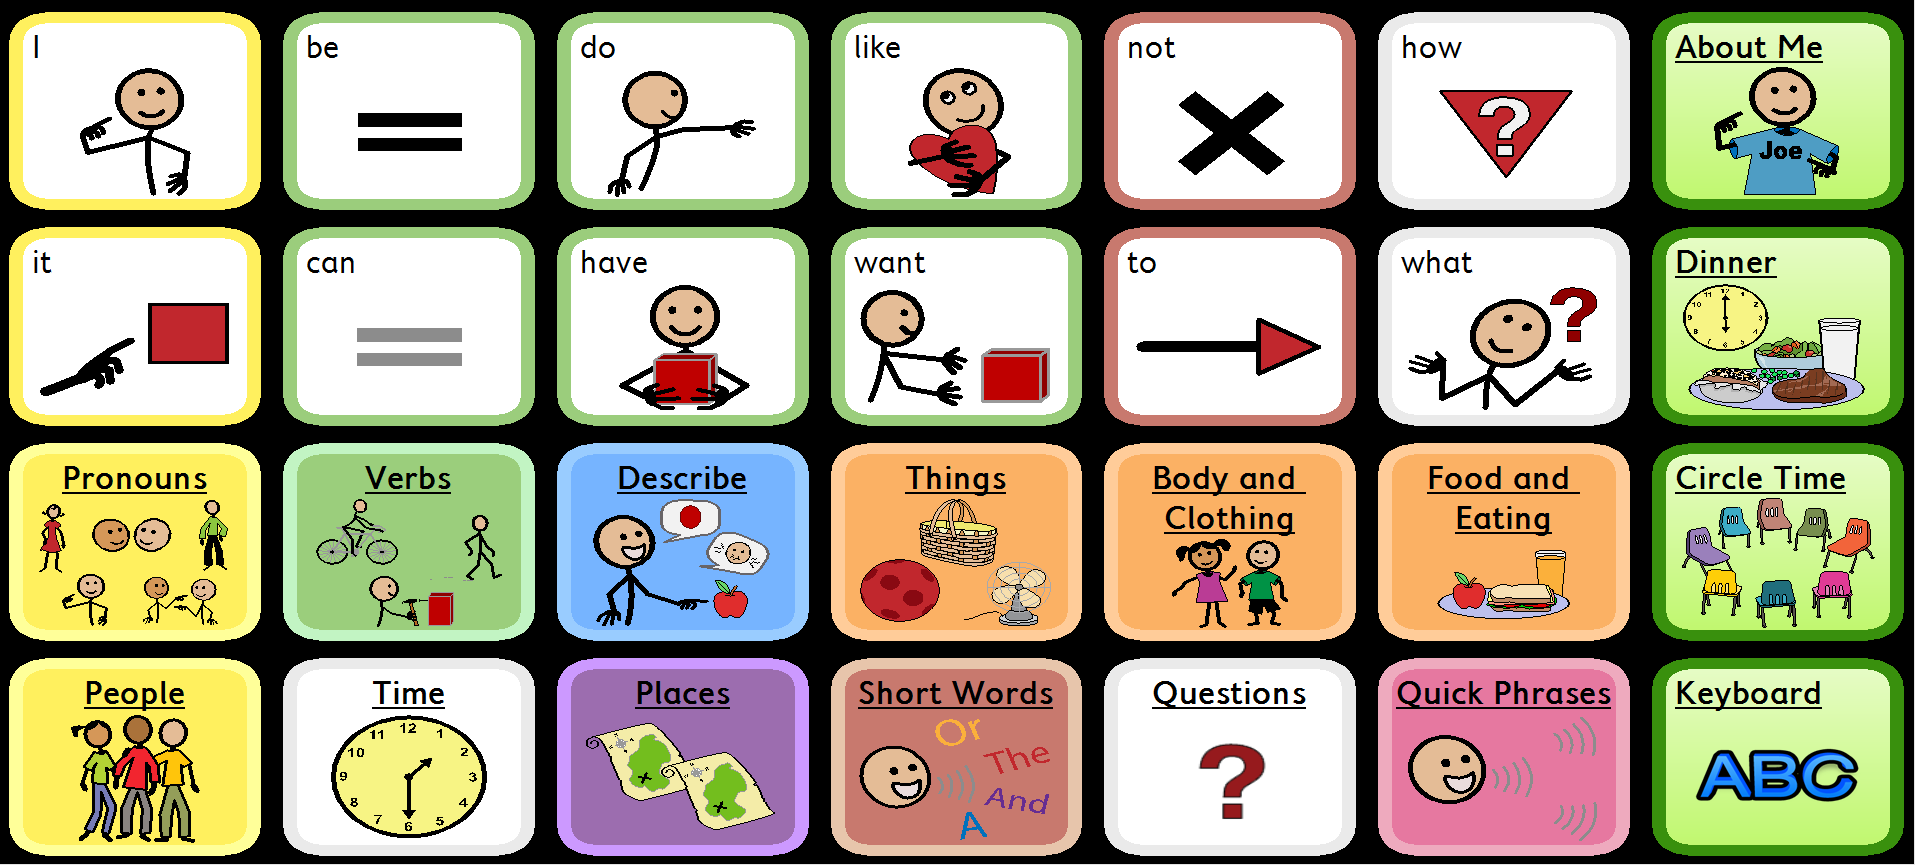
\includegraphics[width=100mm]{symbolgrid}
\caption{Skjermdump av symbolgriden til programvaren Sono Flex}
\label{fig:symbolgrid}
\end{figure}


\subsection{Brukerinteraksjon}

Sono Flex tilbyr to måter for brukerinteraksjon,  mus og øyestyring. Mus fungerer som vanlig ved at brukeren svever med musepekeren over ønsket knapp og venstreklikker for å aktivere. Ved øyestyring må brukeren fokuserer blikket på ønsket knapp en gitt tid for at applikasjonen skal tolke det som et klikk. 

Det som skjer er at med engang brukeren fokuserer blikket på en knapp så starter en nedtelling. Figur \ref{fig:knapp-interaksjon} viser hvordan brukeren presenteres for hvor mye av nedtellingen som gjenstår.  Hvis brukeren ikke flytter blikket før nedtellingen har nådd null tolkes dette som et klikk.
For å gi brukeren beskjed om et godkjent klikk så dannes det en rød firkant rundt knappen. 

\begin{figure}[ht!]
\centering
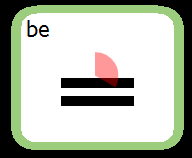
\includegraphics[width=50mm]{Knapp-interaksjon}
\caption{Skjermdump som viser hvordan nedtellingen på en knapp ser ut. Når den røde sirkelen er komplett oppfattes det som et klikk}
\label{fig:knapp-interaksjon}
\end{figure}


\section{Organisasjon og Navigasjon}

Som nevnt i seksjon \ref{subsec:navigasjon} så vil et barns vokabular være så stort at en nødvendigvis må fordele ordene over flere sider. Sono Flex har eksempelvis 106 ord under kategorien "Ting". Med tanke på at det maksimalt er plass til 28 ord på hver side så må disse fordeles og det må finnes en måte å navigere sidene. Løsningen har blitt en svært flat struktur med et hierarki på maksimalt 2 nivåer, ergo det finnes ikke underkategorier. Figur \ref{fig:hieraki-ting} viser hvordan dette fungerer i praksis. Når man trykker på kategorien "ting" så fylles tabellen med 27 ord som passer inn i kategorien "ting". Hvis man ikke finner ønsket ord på den første siden, Navigerer man videre med knappen "neste side" og ordene i tabellen erstattes av nye ord. 


\begin{figure}[ht!]
\centering
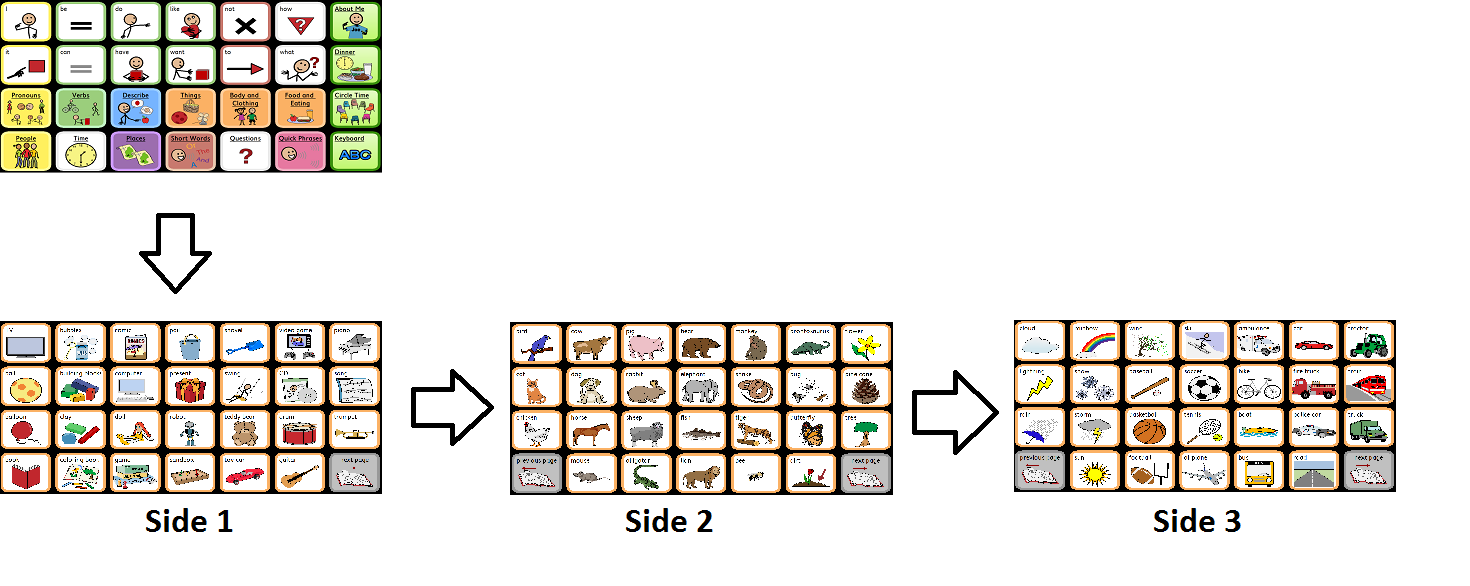
\includegraphics[width=140mm]{Symbgrid}
\caption{Skjermdump hierakiet til Sono Flex}
\label{fig:hieraki-ting}
\end{figure}




\chapter{Utvikling}

I dette kapittelet vil utviklingsfasen bli beskrevet.  


\section{Utgangspunkt}

Denne avhandlingen handler om å forbedre programvaren Tobii Sono Flex som ble forklart i kapittel \ref{chap:Tobii-Sono-Flex}. 
Det mest naturlige ville vært å utvidet eksisterende kode med nye funksjonalitet,  men begrensninger på gjeldene eksisterende gjorde dette vanskelig. Utviklingen ble derfor startet med blanke ark. 


\section{Teknologier}

Øyesporingsenheten beskrevet i kapittel  krever at systemet kjører på operativ systemet Windows og APIet som det leveres enheten leveres med,  fungerer kun i programmeringspråkene C\# og C++. Med dette som utgangspunkt ble resten av teknologivalgene er basert på anbefalinger fra dokumentasjonen og tidligere erfaring. 

\begin{description}
  \item[IDE] Visual Studio
  \item[Rammeverk] .NET
  \begin{description}
     \item[Programmeringspråk] C\#
     \item[Grafikk] Windows Presentation Foundation 
\end{description}
  \item[Versjonskontroll] Git (BitBucket)
\end{description}



\section{Layout}











\chapter{Applikasjon}

\section{Organisasjon}


\section{Animasjon}

\section{Navigasjon}

\section{Personlig tilpasning}

\subsection{Tema}

\subsection{Hurtighet}









\chapter{Dette er bare utkast & stikkord}

Fitzergald key, personliggjør keyboardet med farger. Viktigste er at det er konsistent


For å kunne bruke symboler som en kommunikasjonsform kreves det at brukeren har mulighet til samhandle med dem. For å få til dette brukes det en øyestyringsenhet koblet til en datamaskin som fanger opp brukerens pupill bevegelser. På den måten erstatter øyene den vanlige musepekeren.

\subsubsection{Kalibrering}


Første gang en kobler øyestyringsenheten til maskinen, anbefales det at brukeren gjør en oppmåling og kalibrering for mer presis øyesporing. Oppmålingen innebærer at personen måler størrelsen på skjermen - kalibreringen at det brukeren bes om å følge en prikk som traveserer skjermen. Ettersom dette vil gi øyestyringsenheten et referansepunkt. Prosessen er kun nødvendig første gang for gjeldene bruker. 






Dette gir tilgang på deres application programming interface (API), herved referert til som Tec API. Tec API gjør funksjoner og informasjon fra sporingsenheten tilgjengelig. 


The Tobii Eye Control API provides two alternative access points: a .NET assembly and a C dynamic-link library. Both alternatives
give the developers of eye controlled applications access to the functionality of the Gaze Interaction Server. The .NET API also
contains specialized interaction support for common user interface frameworks such asWindows Presentation Foundation
(WPF) andWindows Forms. The C interface, called MPACI, provides backward compatibility with older Tobii products such as
the MyTobii software.

\Todo{//Hodebevegelser har lite innvirkning på resultatene. Ved å bruke to kameraer., skriv om  3, der kan en lure inn litt om kalibreringen til øyesporingen}


\subsection{Systemkrav}

\subsection{Nøkkelfunksjoner og konsepter}

\section{}

Første gang en kobler til må en gå igjennom ett oppsett. Dette innebærer måling av den aktuelle skjermen som brukes og en kalibrerings rutine. For å oppnå nøyaktig øyesporing.  

For en førstegangsbruker av enheten anbefales det å gjøre en kalibrering, for optimal opplevelse. Informasjonen


Øyestyringsenheten som er illustrert i figur \ref{fig:tobiiPc}  . Denne




\medskip

\bibliographystyle{chicago}%Used BibTeX style is unsrt
\bibliography{sample}

\end{document}
/